
\RequirePackage{lineno} 
\documentclass[,superscriptaddress,showpacs,amssymb,amsmath,amsfonts,linenumbers,article]{revtex4-1}
%\documentclass[prc,preprint,superscriptaddress,showpacs,amssymb,amsmath,amsfonts,aps]{revtex4}
%\setlength{\topmargin}{-1.0cm}
\usepackage{graphicx}
\usepackage{dcolumn}
\newcolumntype{d}[1]{D{.}{.}{-1}} 
%\usepackage{epsfig}
\usepackage{latexsym}
\usepackage{amsmath} 
\usepackage{url}
\usepackage{natbib}

\usepackage{mathtools}
\usepackage{framed}
\usepackage{diagbox}
\usepackage{multirow}
\usepackage{hyperref}
\usepackage{float}
%\restylefloat{table}
\usepackage[margin=20mm]{geometry}
\usepackage{enumerate}



\newcolumntype{C}[1]{>{\centering\arraybackslash}m{#1}}



%\usepackage[dvips]{color}

%\newcommand{\Dfrac}[2]{\frac{\displaystyle #1}{\displaystyle #2}}
%\newcommand{\F}[1]{Figure~\ref{#1}}
\pagenumbering{arabic}
\pdfminorversion=5 
\pdfcompresslevel=9
\pdfobjcompresslevel=9

%
\begin{document}

\begin{center}
\vspace{2cm}
{\Large ANSWERS TO THE FIRST ROUND OF AD-HOC COMMITTEE COMMENTS ON}\\[0.7cm]  

{\bf \large
Measurements of $\gamma_{v} p \rightarrow p' \pi^{+} \pi^{-}$ cross section with the CLAS detector for 0.4 GeV$^2 < Q^2 < 1.0$ GeV$^2$ and 1.3 GeV $< W <$ 1.825 GeV \\[0.7cm]}

by G.V. Fedotov, Iu. Skorodumina, V.D. Burkert, R.W. Gothe, K. Hicks, V.I. Mokeev,\\ and CLAS Collaboration\\[0.5cm]
\end{center}


Ad Hoc Committee: W. Armstrong, N. Markov, M. Ripani (chair)\\[1.5cm] 


\vspace{1cm}
{\bf We would like to thank the Ad Hoc Committee members for their comments and suggestions. Below the answers are listed.  }

\vspace{1cm}


Overall Comments\\[0.5cm]

All committee members agree that the text needs many improvements in terms of wording and in the way results are organized and presented, in order to match the quality of the paper with the quality and impact of the results.\\[0.5cm]

Numbers below refer to lines in the paper.\\[0.5cm]





\vspace{1cm}
\underline{\bf Comments by Whit Armstrong}\\[1cm]

Overall Comments\\[0.5cm]

%----------------\\[0.5cm]

The data analysis behind this paper is very clear and the results are of high quality. As a whole, the content presented in the paper is complete, however, the writing needs *significant work*. The excellent analysis and results deserve an equally high quality presentation.\\[0.5cm]


There were far too many grammatical corrections and improvements for me to note all of them. Here I just make a few comments in addition to the specific comments below.\\[0.5cm]

1. Many grammar and writing issues need to be addressed. Many sentences and paragraphs need to be restructured. Much of the text is phrased in a way that might be OK for an "analysis note" but is insufficient or too informal for publication.\\
{\bf Many changes were introduced into the paper and we hope that now it looks better.}\\[0.5cm]

2. Keep consistent naming, e.g., ``Fig."$->$``FIG." in the text. Also (I could be wrong) I don't think references can be referred to by just the citation, i.e., no ``Ref" is needed: ``Ref. [1]"$->$``[1]"\\
{\bf We looked through several PRC papers and found that it is common to have ``Fig." in the text, but ``FIG." in captions and ``Ref." in citations. ``FIG." in captions comes from the PRC latex style file.}\\[0.5cm]


3. A significant amount of editing and proof reading is needed before publication.\\
\vspace{0.5cm}

Some minor things:\\
\vspace{-0.3cm}

\begin{itemize}

\item ``kinematical" $->$ "kinematic"\\[0.5cm]
{\bf Done.}

\item ``systematical" $->$ ``systematic"\\[0.5cm]
{\bf Done.}

\item For equations with text sub/super scripts, use "\text" (e.g.,\$M\_\{\textbackslash text\{left\}\}\$).\\[0.5cm]
{\bf Done.}

\item Remove white space around figures with ``clip,trim=L B R T"\\[0.5cm]
{\bf The white space was removed in some figures.}

\item Use ``FIG. X" (as it is in the captions) everywhere.\\[0.5cm]
{\bf See the answer to the ``Overall Comments" \#2}

\end{itemize}

\vspace{1cm}

\begin{center}
\large \it Specific Comments\\[0.5cm]
\end{center}

\#\#\# Introduction:\\[0.5cm]

\begin{itemize}

\item 12: The first paragraph is weak.\\[0.5cm]
{\bf The first paragraph is introductory and needed to introduce  to a reader the field of physics: exclusive meson electroproduction.}

\item 26: ``Numerical results" aren't these experimental results ?\\[0.5cm]
{\bf No. The first two paragraphs are introductory. They introduce to a reader the field of physics, the CLAS detector, and the CLAS physics database. In that particular sentence we are talking about all ``Numerical results" that are stored in the CLAS physics database. The reported experimental results are introduced only in the third paragraph.} 

\item Paragraph at 53: I suggest moving much of this ``physics motivation" to the first or second paragraphs in the introduction. Then move on to discuss previous experiments, and ending with the current experiment. Currently it is written in the opposite order.\\[0.5cm]
{\bf The idea of the introduction structure (which was changed a little bit since the starting paper version) is the following. The first two paragraphs are introductory. They introduce to a reader the field of physics and CLAS detector. The third paragraph introduces the data presented here. The fourth paragraph describes previously available data on the subject. The fifth paragraph describes one of the possible options of using these data. The sixth paragraph introduces the JM model. The seventh paragraph stands for the preliminary data interpretation, while the last one introduces the outlook. This structure was chosen since the experimental data themselves are the main focus of the paper.} 


\end{itemize}

\#\#\# Experimental Setup:\\[0.5cm]

\begin{itemize}

\item FIG. 1: This figure is of very poor quality. Everything is too small. A diagram might help in addition to photographs.\\
{\bf The figure was changed.}


\item  100:``The experimental configuration for the current" $->$ "The CLAS magnet configuration...". It is not clear what current means.\\
{\bf The sentence was changed to:\\
\textbf{\textit{``The experimental configuration for the analyzed dataset was the following."}}
}

\item  100: This whole paragraph seems not well structured.\\
{\bf We made the changes in the paragraph and hope that now it looks better.
}


\item  131, 146: Be consistent in naming.``Fig. 2" $->$ "FIG. 2" \\[0.5cm]
{\bf See the answer to the ``Overall Comments" \#2}

\end{itemize}


\#\#\# Exclusive reaction event selection:\\[0.5cm]

\begin{itemize}
\item 159: "To reveal..." Passive voice sentence.\\
{\bf We are sorry, we did not understand the concern. Could you please clarify?}

\item FIG. 3: Axes font is too small. (compare with FIG. 4 which is OK)\\
{\bf The figure was changed.}

\item FIG. 4: Caption is poorly worded. I would avoid saying "efficient enough".\\
{\bf The caption was changed.}

\item 204: The single photoelectron peak isn't "so-called". In this paragraph are you referring to the pions producing a signal in the Cherenkov or is this really uncorrelated (not the same PMT as pion)?\\
{\bf We renamed \textbf{\textit{``single photoelectron peak"}} to the \textbf{\textit{``few photoelectron peak"}}. We also made many changes in this part of the text (see the answers on M. Ripani comments to lines 206-207 and 211-228).\\
The issue you are asking about, was subject to lots of investigations during the CLAS operation era. The main source of the few photoelectron peak contamination was found to be the coincidence of accidental PMT noise with a pion track measured in the DC. More details can be found in Ref. M. Osipenko, A. Vlassov, M. Taiuti,
``Matching between the electron candidate track and Cherenkov counter hit", CLAS-NOTE-2004-020.}

\item Paragraph at 211: What is small and large "relative noise"?\\
{\bf The whole paragraph was rephrased. See also the answers on M. Ripani comments to lines 206-207 and 211-228.}

\item 487: What is this paragraph really trying to say? "The reconstructed data and Monte Carlo events were identically binned." Isn't that enough?\\
{\bf In this paragraph we describe the method of the topology combination. There are several methods to do it: in each multi-dimension bin one can sum up events from all topologies or one can select one topology as preferential based on the maximal efficiency or maximal experimental data statistics. We tested all of these methods and chose the first one.}

\end{itemize}

\#\#\# Cross Section Calculation\\[0.5cm]

Overall, the discussion of variables and binning needs significant rework.\\[0.5cm]

\begin{itemize}
\item 493: "Kinematical Variables" $->$ "Kinematic Variables"\\[0.5cm]
{\bf Done.}

\item 516: "must be used" $->$ Really? Why? Are you sure it "must be used" shouldn't be something like "is easier and conventionally calculated in the c.m frame"?\\
{\bf The sentence is changed to: \textbf{\textit{``The kinematic variables that describe the final hadron state are calculated from the four-momenta of the final hadrons in the c.m.s.."}}}

\item 523: Don't use an itemized list here; keep it in paragraph form.\\
{\bf We prefer to keep it in the itemized form. The reason for that is that the choice of variables is very important and should be emphasized, especially taking into account that the angle $\alpha$ is specific for double-pion kinematics and not familiar for many readers.}

\item 536: The formatting of this list is messy. May try more a standard thing: (i) enumerate the text in the paragraph, (ii) you can use Roman numerals, (iii) or lowercase letters.\\
{\bf We prefer to keep it in a conspicuous form. We personally had many difficulties with these notations during the work in this field. It is especially needed if someone wants to reproduce the results or to compare with them.}

\item FIG. 13: remove the extra white space below the figure. (use the includegraphics[...,trim=0mm 10mm 0mm 0mm,clip,... option)\\
{\bf Done.}

\item TABLE I: The font is too small. Also the table layout is not too good. Try something that looks like this ( note that there are no vertical lines)\\[0.5cm]

$-----------------------------------------------
Number of bins\\
W range M \theta \phi \alpha\\
-------------- ----------------------------
1.3-1.35 GeV 8 6 5 5\\
1.3-1.35 GeV 8 6 5 5\\
1.3-1.35 GeV 8 6 5 5\\
1.3-1.35 GeV 8 6 5 5\\
-----------------------------------------------$\\
{\bf The table was changed.}

\item 593: Why take the central value and correct when you could use the average values of all kinematic variables for each bin? In this way you would report the bin limits and the average kinematic variable's values.\\
{\bf 
This approach was chosen for several reasons. \\
1) To facilitate the comparison with other available double-pion production data that were obtained on a similar grid.\\
2) To keep binning equidistant that is preferable also for the comparison purpose and the model analysis.\\
3) The procedure is rather well established and is usually used in double-pion analyses.
}

\item Equation 12: Drop the ";" at the end and use commas with an oxford comma and an "and" before the fully integrated cross section which logically should be a separate equation from the others.\\
{\bf Done.}

\item FIG. 15: Remove white space and increase figure size.\\
{\bf The figure was changed.}

\item 693: Maybe use "uncertainty" instead of "error", here and in the next few paragraphs.\\
{\bf Done.}

\item 792: "Systematical" $->$ "Systematic"\\[0.5cm]
{\bf Done.}

\end{itemize}


\#\#\# Experimental Results in comparison with the model and previously available data\\[0.5cm]

\begin{itemize}

\item This section title should be simplified. Maybe "Comparisons with Experimental Results"\\
{\bf The title is changed to \textbf{\textit{``Comparison with the model and previously available data"}}}.

\item FIG. 18: This is an example of a graph that should share axes on a grid, which will allow you to make things bigger. The y and x ranges are all identical and there is room to move the annotated Q2 values into each frame.\\[0.5cm]
{\bf Done.}

\end{itemize}

\#\#\# Conclusions and Outlooks\\[0.5cm]

\begin{itemize}
\item 955: "are presented." $->$ ``were reported."\\
{\bf Done.}

\item 973: Is the first sentence telling us anything?\\
{\bf The sentence is changed to:\\
\textbf{\textit{``The cross section extraction procedure has some improvements in comparison with previous studies [3-5]."}}
}

\item 980: Remove "that allowed".\\[0.5cm]
{\bf Done.}
\end{itemize}

\#\#\# APPENDIX\\[0.5cm]

\begin{itemize}
\item FIG. 22: Text is too small. Need to enlarge figure.".\\
{\bf The figure was changed.}
\end{itemize}




\vspace{1cm}
\underline{\bf Comments by Nikolay Markov}\\[1cm]

\begin{enumerate}[A.]

\item The text of the paper has to be proofread.\\
{\bf Many changes were introduced into the paper and we hope that now it looks better.}

\item The novelty and importance of the results can be emphasized more clearly.\\
{\bf Both introduction and conclusion sections were changed.}

\item Could you put more details about the physics you are aiming at? Both introduction and conclusion, what are you looking for and how exactly your data will help.\\
{\bf Both introduction and conclusion sections were changed.}

\end{enumerate}

\begin{itemize}

\item 32 : The cross sections were extracted via the CLAS data analysis. Could you clarify?\\
{\bf The sentence was rephrased in the following way:\\
``\textbf{\textit{ The cross sections were extracted along the standards of the CLAS data analysis ...}}''\\
In this sentence we wanted to emphasize that the data collected with the CLAS detector are analyzed.
}


\item Fig. 1 Figure is not very clear. One can hardly read captions within the figure.\\
{\bf The figure was changed.}

\item 90 ``toroidal magnetic field including mini torus coil" -- could you clarify sentence?\\
{\bf The sentence \textbf{\textit{``The CLAS detector had a toroidal
magnetic field including a mini-torus coil to reduce background from Moeller scattering."}}\\
was changed to \textbf{\textit{``The CLAS detector had a toroidal magnetic field that bended charged particle trajectories and therefore allowed to determine their momenta in DC."}}
}

\item 106 ``non-signal events" -- what is it?\\
{\bf \textbf{\textit{``non-signal"}} was changed to \textbf{\textit{``background"}}}.

\item 129 you talk about beam offset without explaining what it is.\\
{\bf An explanation footnote was added.}

\item 159 you need DC in order to calculate sampling fraction.\\
{\bf The clarification sentence was added into the second paragraph of this subsection.}

\item 252 TOF system provides timing information for tracks, T.\\
{\bf The sentence was changed.}

\item 256 you are talking about TOF paddels without introducing them.\\
{\bf We changed throughout the text the word \textbf{\textit{``paddle"}} to the \textbf{\textit{``scintillator"}} or \textbf{\textit{``scintillator counter"}}, which are of more common use. We also refer to the paper ``B. A. Mecking et al., Nucl. Instr. and Meth. 503, 513
1068 (2003)", where a reader can find the details of CLAS design.}

\item 392 you introduce DAQ livetime without explanation. The whole ``Quality Check cut" part is full of technical details.\\
{\bf DAQ livetime is explained at the beginning of the third paragraph of the section. This ``Quality Check cut" is the feature of the analysis that we would like to emphasize. It is equivalent to the so-called ``golden run selection", but it is done more precise on a level of blocks. We have already squeezed the section in comparison with that in the Analysis note and kept only relevant details that are needed for understanding of the procedure.}

\item 501 - 519 do we need such a detailed explanation of the frames of references?\\
{\bf The idea of such detailed explanation is to provide a reader with a full recipe of the procedure. It is especially important if the reader would try to reproduce or compare with our results. We personally had difficulties with that during the analysis, since such details are usually skipped.   
}

\item Page 9, Binning and kinematical coverage. The discussion of binning in invariant mass is very important but slightly confusing as of now. Can possibly adding an illustration from the data make it more clear?\\
{\bf During the analysis we encountered difficulties with proper binning in invariant masses. We investigated this issue for a long time and developed an appropriate procedure of that. We decided to include these details into the paper to help other people which may encounter the same difficulties.
}

\item Page 9, Binning and kinematical coverage. Is it possible to add a sample plot with angular coverage in one of the topologies?\\
{\bf 
\begin{figure}[htp!]
\begin{center}
 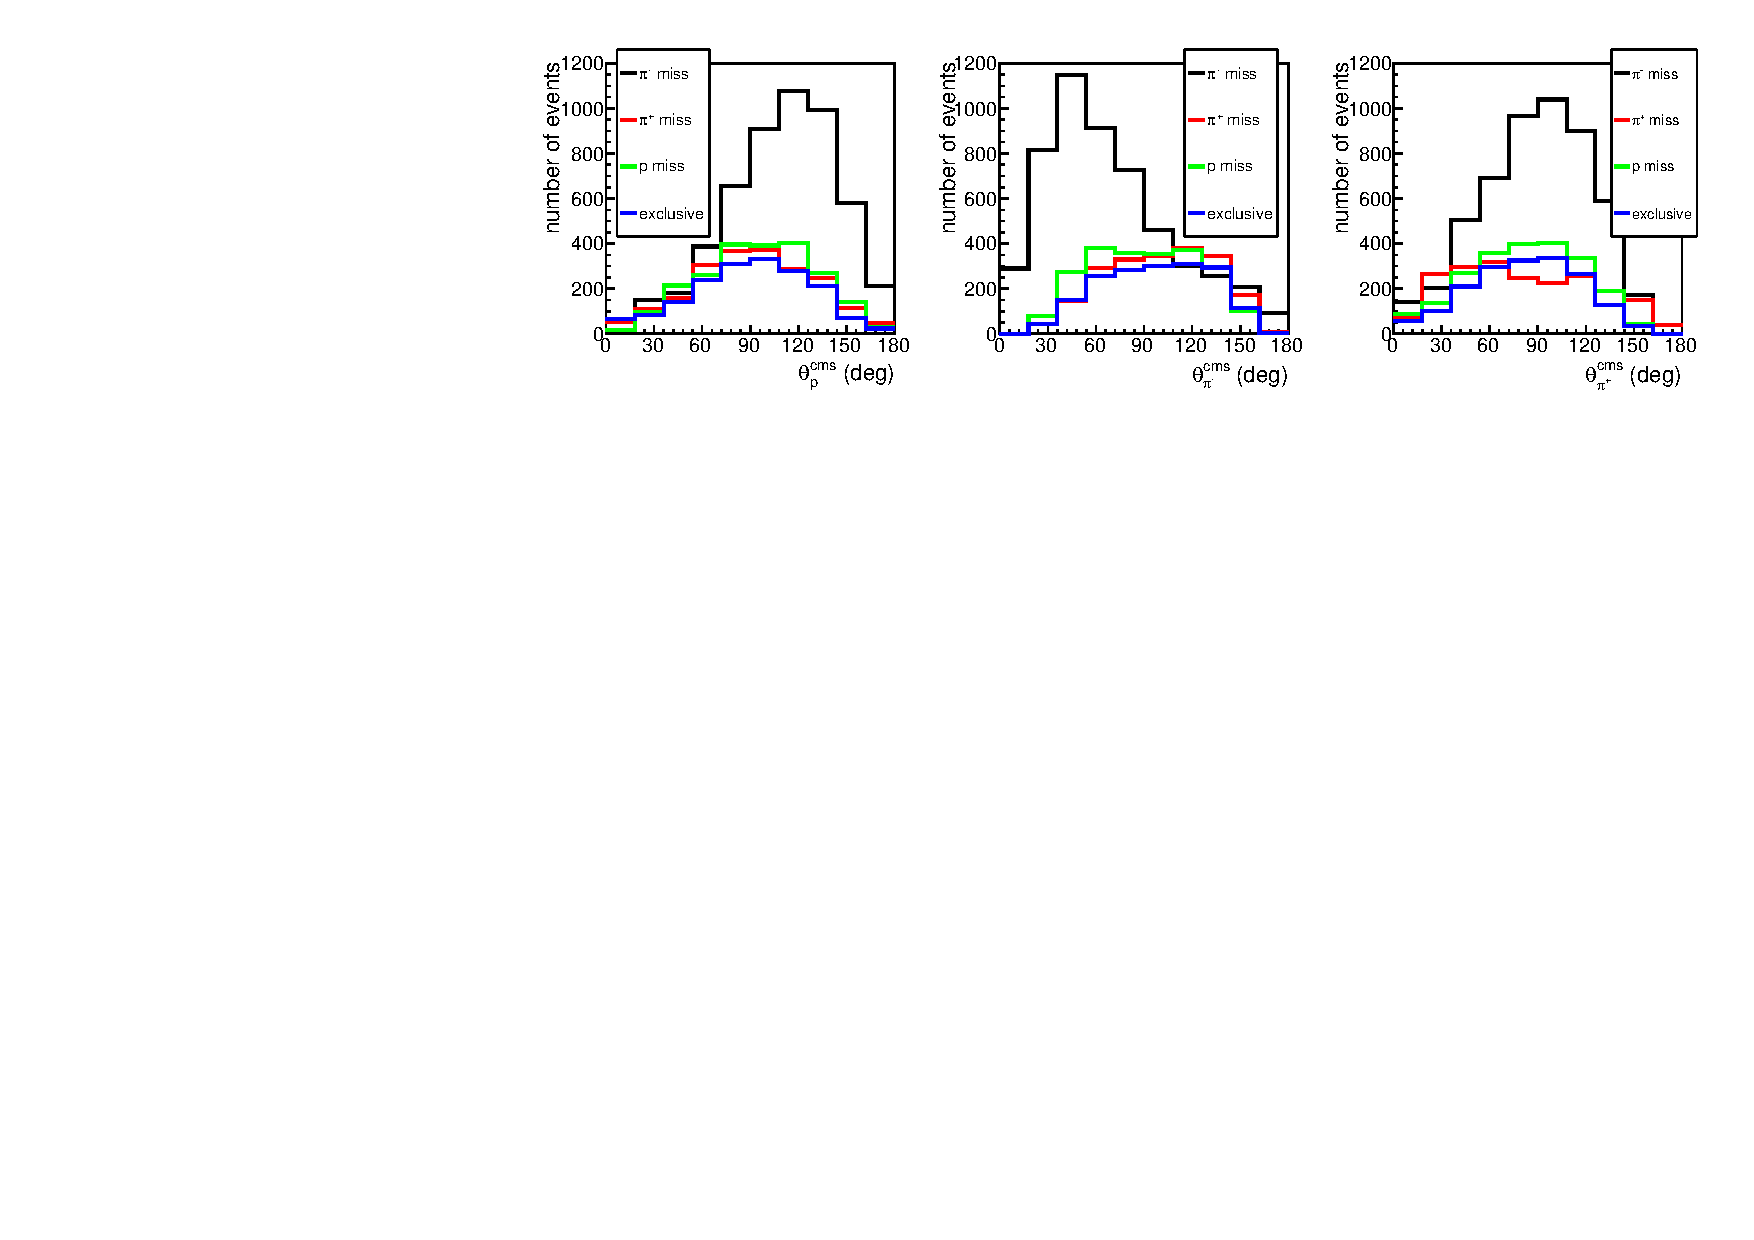
\includegraphics[width=14cm,keepaspectratio]{pictures/theta_var_top.pdf}
 \caption{\label{ang_cover}}
\end{center}
\end{figure} 
}
{\bf The comparison of the experimental event yields for various topologies as functions of the $\theta^{\text{cms}}$ angles is presented here in Fig.~\ref{ang_cover} for $Q^{2} = 0.475$~GeV$^2$ and $W = 1.6125$~GeV. As it is seen from the figure, at extreme angles the other topologies give contributions that are comparable with that for the $\pi^{-}$ missing topology. This is why it is important to combine various topologies. But even with the combination of the topologies the extreme points have a lot of ``empty cells" and therefore large error bars are associated with them.\\
We prefer to not include these plots into the paper since they are not informative and may confuse the reader. To be more informative, the event yields should be divided to $\Delta cos(\theta)$ and corrected to the detector acceptance. But in this case the plot will loose the information about number of events in each topology.}



\item Chapter 4, subchapters B, C, D: you mention two different event generators, TWOPEG and GENEV, with different models (JM15 and JM05) which are seemingly used for different purposes. Could you use the same generator everywhere?\\
{\bf Unfortunately, the TWOPEG event generator did not exist at the time when the simulation was carried out. The full double-pion simulation requires a lot of time (years) and consumes a lot of space on tapes. This is why the simulation was not redone with TWOPEG. Beside that, GENEV has proven itself as an efficient tool for the efficiency evaluation in previous analyses.

Taking into account the fact that TWOPEG is more advanced event generator, which better describes the available data and allows to obtain the absolute cross section value, it was decided to use it for the purpose of radiative corrections and estimation of the empty cell contribution. 
}

\item Fig 16. On your plot of the cross sections angular dependence (Fig. 16) one can see error bars only at extreme points over angles. Moreover, there are no error bars visible when you do not use contribution from empty cell.\\
{\bf In Fig.16 for the open squares (ignored empty cell contribution) the error bars correspond to the uncertainty $\delta_{\text{stat}}^{\text{tot}}$ given by Eq.~(18) and are smaller than the symbol size. For black points (empty cell contribution taken into account) the error bars correspond to the uncertainty $\delta_{\text{stat,mod}}^{\text{tot}}$ given by Eq.~(19). They are seen mostly at the extreme points over $\theta$ angle  due to the complete absence of the CLAS acceptance in the corresponding directions. The caption is changed accordingly.\\
The fact that the statistical uncertainty is so small that it is not visible, was emphasized in the text (see Sect. V, third paragraph).
}

\item Fig. 18 Is rather hard to read, TWOPEG predictions are completely shadowed by the data points. Systematical uncertainty is presented twice, in the error bars and the black band.\\
{\bf Fig. 18. was changed.
}

%The data symbols are enlarged and changed to open circles, while the TWOPEG curve is made thinner. The error bars correspond to the total uncertainty which is statistical and systematical ones summed up in quadrature, while the bands stand for the systematical uncertainty only.

\item Barn symbol is b, not bn.\\
{\bf Done.}

\item Fig 21. Is rather hard to read, symbols overlaps.\\
{\bf Fig. 21. was changed.}
%The ``e1e" data symbols are enlarged and changed to open circles.

\item In your comparison with the model you compare full cross sections with the TWOPED results and get the resonance part from the JM. Why you do not get the full results from the JM?\\
{\bf The reason for that is the following. It is rather easy to calculate the resonant part in JM model. To obtain full cross sections from the JM model, one needs to perform a model fit, which is a separate and rather complicated task that includes establishing non-resonant mechanisms. The fit procedure may take a long time (years) and will be the subject of a future publication from the phenomenologists/theorists side. In this paper we just would like to emphasize that the obtained data are of interest for a phenomenological/theoretical analysis.  
}


\end{itemize}





\vspace{1cm}
\underline{\bf Comments by Marco Ripani}\\[1cm]

\begin{itemize}


\item 26 - This sentence could be placed in a footnote, keeping the reference [2]\\
{\bf Done.}

\item 50 - It is true that a different averaging makes the comparison less meaningful, but nevertheless such a comparison should be shown as further reassurance that old and new data are compatible

\begin{figure}[htp!]
\begin{center}
 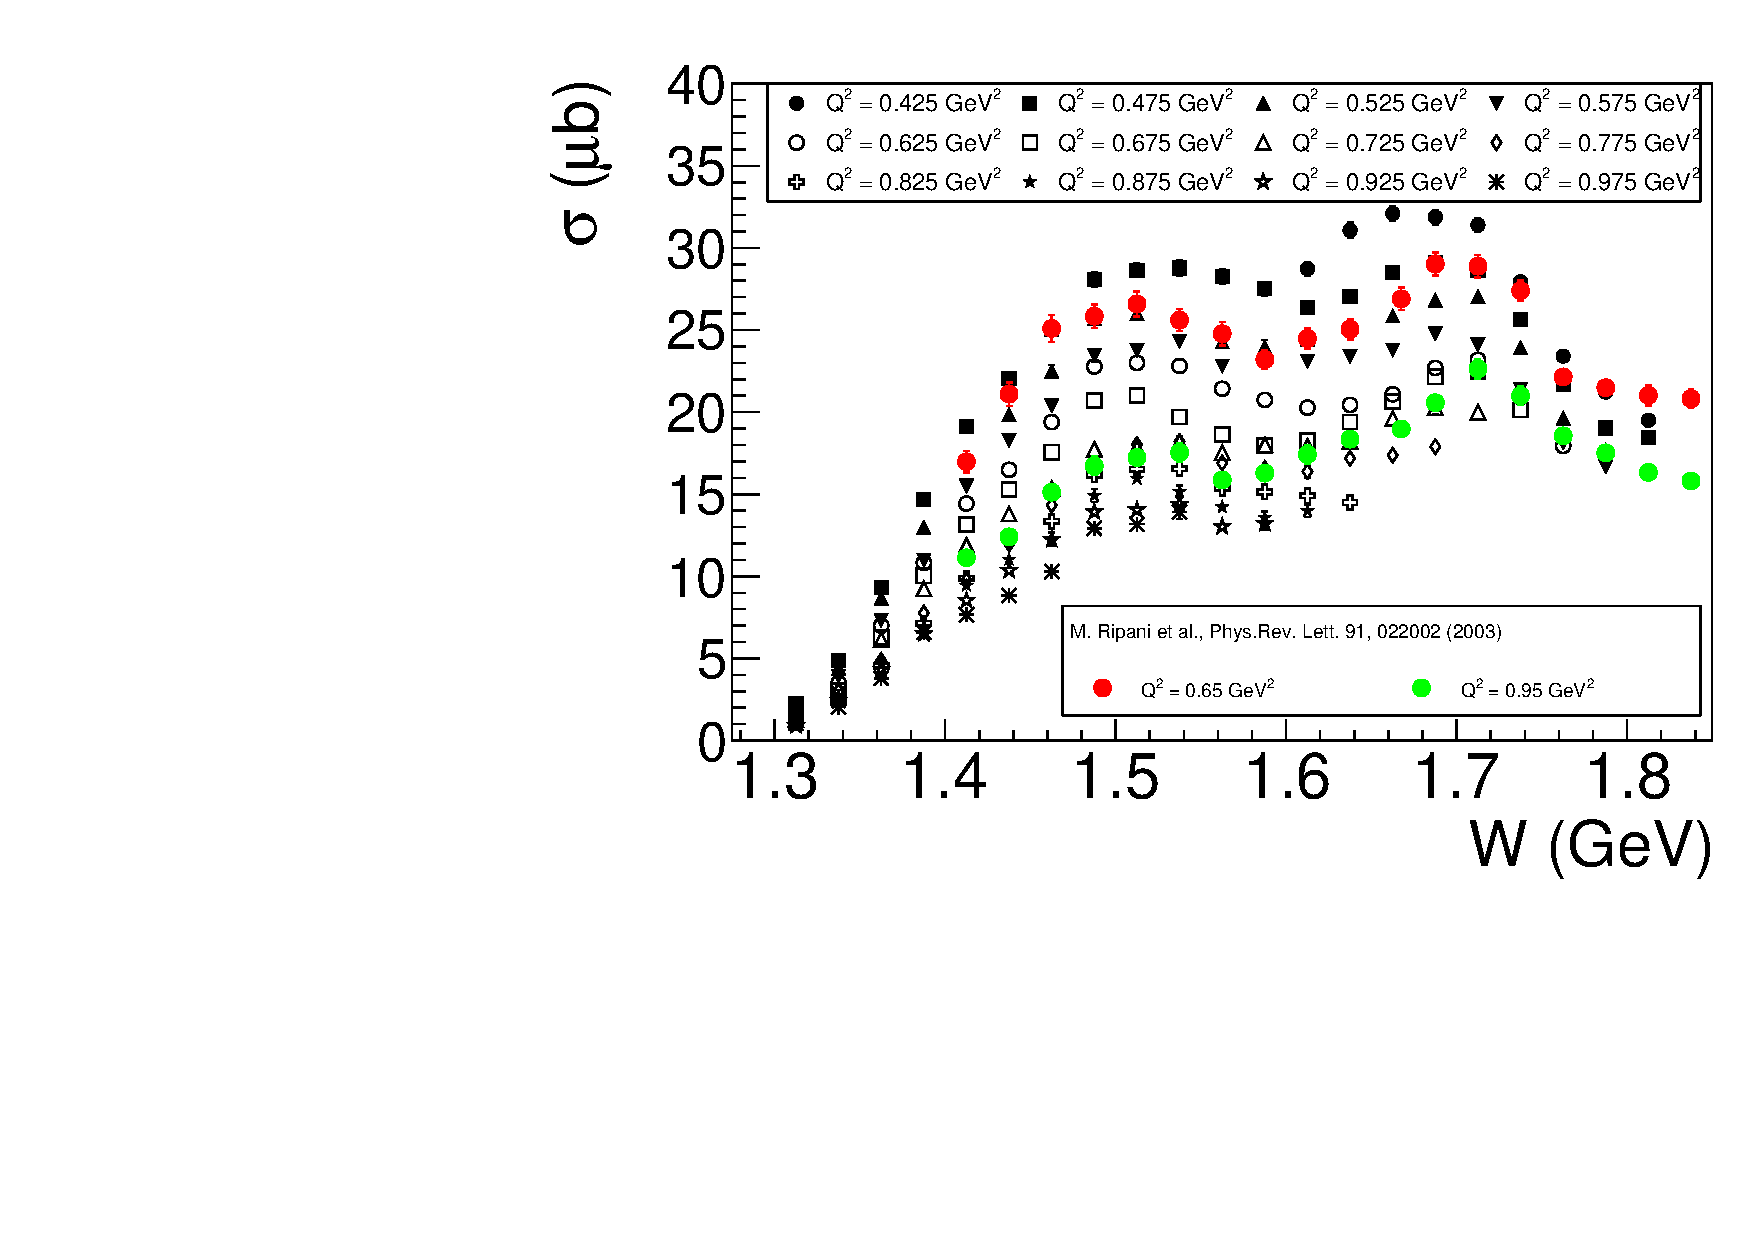
\includegraphics[width=14cm,keepaspectratio]{rip_compare.pdf}
 \caption{\label{rip_compare}}
\end{center}
\end{figure} 

{\bf
This comparison is shown here in Fig.~\ref{rip_compare}. As it is seen, it is rather hard to interpret it due to the interplay of two factors: 6-times larger bin size and different beam energies. So we decided to not include it into the paper in order to not confuse a reader. We rephrased the part of the introduction where these data are mentioned in more careful way.
}


\item 56 - ``resonance manifestation" $-->$ "resonances above the Delta(1232)" or "resonances above the first excitation region"\\
{\bf Done.}


\item 67 - ``has proven itself" $-->$ ``has proven effective"\\
{\bf The sentence is changed to:\\
\textbf{\textit ``This model, aiming at the extraction of resonance electrocouplings and the identification of different reaction mechanisms, has proven itself as an effective tool for the analysis of the experimental cross sections~[6-8]."}}

\item 80 - ``with masses up to 1.8125 GeV" $-->$ there is no need here to give such a precise value, 1.81 GeV can suffice\\
{\bf Done. Changed to \textbf{\textit ``up to $\sim$1.8~GeV"}}.

\item 89 ~~Electromagnetic Calorimeter" $->$ ``sampling Electromagnetic Calorimeter"\\
{\bf Done.}

\item 100-102 ``The experimental configuration for the current, called ``e1e" dataset was the following. The torus current was 2250 A and the mini torus current 5995 A."$->$ There is no need to give this data here, as they are not very meaningful to the reader. You can just say something like ``The torus field setting was such as to bend electrons away from the beamline (outbending configuration)."\\
{\bf We agree that sentence needs rephrasing, however the negative particles were inbending in this run configuration. The new sentence is: \textbf{\textit{``The torus field setting was such as to bend negative particles toward the beamline (inbending configuration)."}}.
}

\item 108-117 This is a detailed and unnecessarily long explanation. You can just say that ``In order to avoid bubble formation due to the specific e1e experimental conditions, the target had a special conical shape that allowed draining the bubbles away from the beam interaction region."\\
{\bf We agree. The part of the text: \textbf{\textit{``It had a conical shape ... thus clearing the beamline."}}\\
was changed to: \textbf{\textit{``In order to avoid bubble formation, the target had a special conical shape that allowed draining the bubbles away from the beam interaction region."}}
}

\item 129 ``non-signal" $->$ ``background"\\
{\bf Done.}

\item 134 ``corresponded" $->$ ``corresponding"\\[0.5cm]
{\bf Done.}

\item 145 ``in Fig. 2, events" $->$ ``in Fig. 2: events"\\
{\bf Done.}

\item 174-176 ``the deposited.....($P_{e}$)," $->$ ``by design the energy deposited in the active scintillators $E_{tot}$ is about 1/3 of its momentum $P_{e}$," Remember above we added the specification ``sampling" calorimeter, so its composition should be rather obvious, although the showering part may be different from lead. But here it is irrelevant.\\
{\bf The third paragraph in this subsection was rephrased according to the suggestion (see the three last sentences).}

\item 181-182 ``since.....sheets" $->$ remove, based on the above sentence it is not necessary anymore\\
{\bf See the answer on the previous question.}

\item 196 ``below than that" $->$ ``below that"\\[0.5cm]
{\bf Done.}

\item 206-207 and 213-214 It is said that the CC spectrum shows a ``so-called single photoelectron peak, which was actually located at a few photoelectrons." but then it is said that the noise results in a ``very pronounced single photoelectron peak". Is it one or a few photoelectrons ? You should be consistent here.\\
{\bf We replaces \textbf{\textit{``single photoelectron peak"}} to \textbf{\textit{``few photoelectron peak"}} everywhere}.


\item 211-228 All the text here is somewhat confusing. One thing is the single or few photoelectron noise, the other is that low-efficiency regions feature a photoelectron distribution which is shifted towards zero and therefore adds up to the ``single" or ``few" photoelectron region. The whole paragraph should be replaced by
something like ``Signals from inefficient Cherenkov regions are depleted of good events, as shown in Fig. 4 (the inefficient area in the middle of a sector was expected since two CC mirrors were joined there). Therefore appropriate fiducial cuts were developed to exclude those regions from the analysis".\\
{\bf We changed the beginning of the paragraph and hope that now the explanation is clear.}\\[0.5cm]

Also, it is not clear why the distribution shown in Fig. 4 should be specific to e1e, in what sense ?\\
{\bf We added that sentence since in the analysis of this particular dataset we were not able to reproduce elastic cross section without this specific cut. But you are right, the procedure is applicable to any dataset, so finally we decided to remove this sentence.}\\[0.5cm]

Finally, it would be better to be more quantitative as to the criteria to define an efficient vs an inefficient. So, the final two sentences in the paragraph should read as something like ``The curves which are superimposed on the distribution show an overall fiducial cut that is applied in the CC plane. Then, within that overall cut, for both experimental data and Monte Carlo simulation, only electron candidates that originated from black regions within the fiducial cut were analyzed, where the black regions are defined as those having an average photoelectron number greater than ?????". The latter definition could be repeated in the caption of Fig. 4.\\
{\bf We change the end of the paragraph according to the suggestion, excluding the explanation of how exactly the black regions were defined. The procedure of their definition is described in the Analysis note. This procedure is more complicated than just the cut on the average photoelectron number. We cut on the ratio ``number of events with more than 5 photoelectrons" over the ``total number of events". So we decided to skip this long explanation in order not to confuse the reader. }\\[0.5cm]


Question, where the requirements (I guess described in [10]) of matching between track and geometrical PMT position, as well as time coincidence between CC, TOF and EC hit applied here ? If not, why ? Were they applied, thus leading to Fig. 5 ?\\
{\bf It was found that after inefficient zones removal the influence (either on total statistics and on events from few photoelectron peak) of the mentioned above cuts and corrections is insignificant. So, the standard procedure of cutting out this peak, fitting by Poisson etc. is needed anyway.}

\item 231 ``presented" $->$ ``present"\\[0.5cm]
{\bf Done.}

\item 263 ``corresponded" $->$ ``corresponding"\\[0.5cm]
{\bf Done.}

\item 265 ``corresponded" $->$ ``corresponding"\\[0.5cm]
{\bf Done.}

\item 278-280 ``To cure that effect, a special procedure to correct the timing information provided by the TOF was used." $->$ ``A special procedure was developed to correct the timing information for the affected paddles."\\
{\bf The sentence was changed accordingly.}

\item 329-335 ``However, in order to avoid shifts in distributions of some kinematical quantities (e.g. missing masses) from their expected values, an energy loss correction was applied to the proton momentum magnitude (both experimental and reconstructed Monte Carlo), since the low-energetic protons were affected the most by energy loss in materials." $->$ ``However, the Monte Carlo cannot perfectly describe all materials in the detector assembly and this could impact in particular the low-energetic protons that are affected the most by energy loss in materials. Therefore, in order to correct the shifts of specific missing mass distributions from their expected values, an energy loss correction was applied to the proton momentum magnitude (both experimental and reconstructed Monte Carlo)"\\

{\bf There is a misunderstanding here. We trust the way the detector simulation propagates particles through the media. And our correction is fully based on that simulation. The only reason to establish and apply this correction was to have the positions of the peaks in distributions (such as missing masses) on the expected places. The explanation sentence is added to the end of the paragraph.}

\item Fig. 7, legend $->$ ``befor" $->$ ``before"\\
{\bf Done.}

\item 345-353 ``Moreover, the edges of the detection area do not provide a safe region for particle registration, being affected by rescattering from the coils, field distortions, and similar effects. Therefore it is now a common practice to consider only those particles that were found in "safe" areas inside specific fiducial cuts, i.e. cuts on the kinematic variables (momentum and angles) of each particle. These cuts were applied for both real events and Monte Carlo reconstructed events." $->$ ``Moreover, the edges of the detection area, being affected by rescattering from the coils, field distortions, and similar effects were excluded from the analysis by applying specific cuts on the kinematic variables (momentum and angles) of each particle. These cuts were applied for both real events and Monte Carlo reconstructed events."\\
{\bf The sentence was rephrased according to the suggestion:\\
\textbf{{``The edges of the detection area, being affected by rescattering from the
coils, field distortions, and similar effects should be excluded from consideration by applying specific (fiducial) cuts on the kinematic variables
(momentum and angles) of each particle. These cuts were applied for both real events and Monte Carlo reconstructed events."}} }

\item 354-356 According the a comment above, the torus setting should have been already described before. No need to repeat it here. ``For that type of particles," $->$ ``For negative, outbending particles (pions in this case), "\\
{\bf We think that it is better to remind a reader the magnetic field configuration here because it has a significant impact on the shape of $\varphi$ vs $\theta$ distributions and fiducial cuts. This paragraph is related not only to pions, but also to electrons. 
}

\item 360-361 ``CLAS sector one in one slice over particle momentum" $->$ ``CLAS sector 1 in a specific momentum slice" sounds better\\
{\bf Done.}

\item 362-365 ``The solid black curves correspond to the applied fiducial cuts. These cuts isolate the regions with a relatively stable yield of events along the azimuthal angle." $->$ ``The solid black curves correspond to the applied fiducial cuts, that select the regions with a relatively flat particle density along the azimuthal angle."\\
{\bf Done.}

\item 371 ``with a relatively stable event yield along" $->$ ``with a relatively flat particle density along"\\
{\bf Done.}

\item 394 ``the FC charge updated" $->$ ``the FC charge was updated"\\[0.5cm]
{\bf Done.}

\item Fig. 11, middle and bottom plots are interchanged in the caption. BTW, the middle plot (inclusive, right ?) shows a kind of double structure, any idea about what is causing this effect ? Here you should show the ratio in middle and bottom plot as points as a function of block number, with their statistical error, which gives a much better idea of whether the event rate is regular and about where to cut. Moreover axis labels and numerical labels are too big, with some overlapping. On the x axis, the tick marks corresponding to the numerical labels are not visible.\\
{\bf The caption and the figure are changed accordingly. You are right, the 2D plots of these quantities as a function of block number are more informative. They were used to establish this cut. They are given in the Analysis note on page 34, Fig. 3.8. The reason why we do not include them into the paper is the following: due to the enormous amount of blocks (significantly more than screen or paper resolution) all of them can not be made visible in 2D histogram. The averaging over some group of blocks or plotting just some of them contradicts the idea of this approach. The more we are averaging, the closer we are to the standard procedure of ``golden run selection". That is why we decided to provide only $y$-axis projections of these distributions. The double structure can be seen as a shift in 2D plots from the analysis note. We do not know the origin of this structure, but may be something changed when the data taking was resumed after the Christmas break.   
}


\item 424 ``to acquire only about 10\% of that." $->$ ``to account only for about 10\% of the total."\\
{\bf Done.}

\item 433 ``Electrons, being very light and rapid," $->$ Electrons, having generally a very high momentum,"\\
{\bf Done.}

\item 472 ``corresponded" $->$ ``corresponding". Same in Fig. 12 caption. Moreover, the panels in Fig. 12 have too big axis labels and numerical labels, with some overlapping. On the x axis, the tick marks corresponding to the numerical labels are not visible.\\
{\bf Done.}

\item 499 ``$y_{lab}$ - up" $->$ "$y_{lab}$ - pointing upwards with respect to the Hall floor"\\[0.5cm]
{\bf Done.}

\item 505 ``virtual photon" $->$ "virtual photon exchanged in the scattering"\\
{\bf Done.}

\item after 558 (why do line numbers disappear in this portion of text ?) ``distribution depend" $->$ ``distributions depend"; ``and the assumed W" $->$ ``and W"\\[0.5cm]
{\bf Done.}

\item Eqn. 11 Where is the photoelectron correction factor $F_{ph.el.}$ ? And here the efficiency correction from the Monte Carlo is called with the same letter $F$. It would be better to show explicitly the factor $F_{ph.el.}$ and use a different name for the Monte Carlo efficiency.\\
{\bf We changed the notation for Monte Carlo efficiency from $F$ to $\mathcal{E}$ throughout the text. Regarding $F_{ph.el.}$, we do not include it in Eqn. 11, since it depends on CC PMT number, while the other factors in Eqn. 11 depend on kinematical cell $\Delta W \Delta Q^{2} \Delta^{5}\tau$. We tried to keep the generality of  Eqn. 11, while the factor $F_{ph.el.}$ is too specific for the experiment. So, we mention this factor in the variable explanation part after the formula.}

\item 658 ``GENEV which assumes" $->$ ``GENEV assumes"\\
{\bf Done.}

\item 661-667 It would have been better to choose for Fig. 12 a kinematic bin where some of the 3 pion background was visible on the bottom panel\\
{\bf We have chosen this bin as a typical one. As it is mentioned in the text the $3\pi$ background for $W>1.6$~GeV grows and become a few percent at $W \approx 1.8$~GeV. But in the analysis we have only two kinematical bins with $W > 1.8$~GeV (at $Q^{2} = 0.425$~GeV$^{2}$ and $Q^{2} = 0.475$~GeV$^{2}$). Beside that, even in those two bins the $3\pi$ background is barely seen (see Fig. 3.13 on page 38 of the Analysis note).   
}

\item Fig. 16. The top-left legend with the $W$ and $Q^2$ bin was drawn with a too small font, you should increase the font size.\\
{\bf The legend is removed, since the same information is given in the caption.}

\item 729-730 ``pronounceable" $->$ ``pronounced"\\[0.5cm]
{\bf Done.}

\item 732-733 ``To account for the possible discrepancies with the model," $->$ ``To account for the model-dependence"\\
{\bf We changed\\
 \textbf{\textit{``To account for the possible discrepancies with the model, the part of the cross section that came from the empty cells was assigned with a 50\% relative error. Finally this additional error was combined with the total statistical one."}} to\\
 \textbf{\textit{``To account for the model dependence, the part of the cross section that came from the empty cells was assigned a 50\% relative uncertainty. The corresponding absolute uncertainty $\delta_{\text{model}}$ was combined with the total statistical one, as it was done in [12,22]"}}\\
Here we introduced a new variable $\delta_{\text{model}}$ (see also Sect IV.F) in order to properly explain the reported cross section uncertainty.
 }

\item 734 ``was assigned with a 50 \%" $->$ ``was assigned a 50 \%"\\[0.5cm]
{\bf Done. }

\item 740-741 ``which accounts the radiative" $->$ ``which accounts for the radiative"\\[0.5cm]
{\bf Done.}

\item 748 ``colliniarly" $->$ ``collinearly"\\[0.5cm]
{\bf Done.}

\item 760 remove the comma after ``electroproduction"\\[0.5cm]
{\bf Done.}

\item Formula (16) there is an extra bracket ) after $delta_{F}$\\[0.5cm]
{\bf Done.}

\item 794-795 ``from the several sources" $->$ ``from several sources"\\[0.5cm]
{\bf Done.}

\item 800 ``was revealed" $->$ ``was found"\\[0.5cm]
{\bf Done.}

\item Section G. Wasn't any systematic error assigned to the differential cross sections ? The paper only mentions systematic errors on the integral cross sections and there is comment/explanation as to why no such error was calculated for the differential ones. A few words of explanation are in order.\\
{\bf We added the following sentence to the end of the section IV.G:\\
\textbf{\textit{``The relative systematic uncertainty in each $W$ and $Q^{2}$ bin can be propagated as a global factor to the single-differential cross sections, which are reported with the uncertainty $\delta_{\text{stat,mod}}^{\text{tot}}$ defined by Eq. (19)"}}\\
}
 
%We report 4 sources of systematical uncertainties. Three of them can hardly be estimated as a function of the final hadron variables. The uncertainties due to the normalization verification and radiative correction are assigned to the cross section as global factors. Beside that, the uncertainty due to the integration over various kinematical grids can be determined only as a function of $W$ and $Q^{2}$. And only the uncertainty due to the topology combination may be estimated as a function of final hadron variables, but it has the smallest contribution to the total systematical uncertainty.

%This is why we decided to report the systematical uncertainties only in $W$ and $Q^{2}$ bins. If one needs the systematical uncertainty for the differential cross section, one may take the relative uncertainty for the given $W$ and $Q^{2}$ bin and apply it as the same factor for each point of the differential cross section distribution. 


\item Fig. 19 There are no errors on the data points, while there is an error on the corresponding W point in Fig. 18....\\
{\bf Previously the error bars in Fig. 18 corresponded to the total uncertainty ($\delta^{\text{tot}}_{\text{stat,mod}}$ given by Eq.~(19) summed up in quadrature with the total systematic one), while in Fig. 19 they corresponded to the $\delta^{\text{tot}}_{\text{stat,mod}}$ only.\\
Now Fig. 18 is changed in a way that error bars also correspond to the $\delta^{\text{tot}}_{\text{stat,mod}}$, however they are smaller than the symbol size. We also added the following explanation to the third paragraph of section V: 
\textbf{\textit{``The extracted cross sections benefit from the minimal statistical uncertainty (as well as model dependence) among the previous studies of double-pion electroproduction cross sections~[3-5]. This was achieved due to high experimental statistics and the fact that four reaction topologies were  analyzed in combination."}}
}

\item 861 ``It aims at extracting of the resonance" $->$ ``It aims at extracting the resonance"\\[0.5cm]
{\bf Done.}

\item 908 ``high laying" $->$ ``high lying"\\[0.5cm]
{\bf Done.}

\item 958-960 ``The results were obtained.........in a kinematical region that lacked information on double-pion cross sections" $-->$ as said a few lines after, there is overlap with both Ref. [3] and Ref. [4], so this statement should be modified. You should say something like ``The results, improve significantly previously available data in this kinematic region either by extending the $W$ coverage or by increasing statistics, thereby achieving a finer binning in $Q^2$ (0.05 GeV$^2$)."\\
{\bf Done.}

\end{itemize}


\begin{center}
\large \it Other things: \\[0.5cm]
\end{center}

\begin{itemize}
\item  Replace everywhere ``sector one" with ``sector 1"\\
{\bf Done.}

\item  Same when you describe the topologies, everywhere in the text replace ``topology one" with ``topology 1" etc.\\
{\bf Done.}

\item  It seems me that we typically talk about ``systematic errors" rather than ``systematical errors" but perhaps they are both valid english expressions, not sure\\[0.5cm]
{\bf We changed ``systematical'' to ``systematic'' everywhere in the text.}

\item  Ref. [9] Egian $->$ Egiyan\\[0.5cm]
{\bf Done.}

\end{itemize}

\end{document}
